
\documentclass[conference]{IEEEtran}

\usepackage{booktabs}
\usepackage{algorithmic}
\usepackage[ruled, vlined, linesnumbered]{algorithm2e}
\usepackage{mathtools}
 \let\labelindent\relax
\usepackage{enumitem}
\usepackage{epstopdf}
\usepackage[utf8x]{inputenc}
\usepackage{amsfonts}
\usepackage{amssymb}
\usepackage{amsthm}
\usepackage{amsmath}
\usepackage{hyperref}
\usepackage{balance}
\usepackage{todonotes}
\usepackage{floatrow}
\usepackage[centerlast,small,sc]{caption}
\usepackage{subcaption}

\floatsetup[table]{capposition=top}

\usepackage{cleveref}
\newcommand{\crefrangeconjunction}{--}
\newcommand{\td}{\todo[inline]}
% correct bad hyphenation here
\hyphenation{op-tical net-works semi-conduc-tor}

\graphicspath{{images/}{./}} % Specifies where to look for included images

\newcommand{\addfigure}[4]{
\begin{figure}[fh]
	\centering
	\includegraphics[width=\linewidth]{#2}
	\caption{#3}
	\label{#4}
\end{figure}
}

\begin{document}
%
% paper title
% can use linebreaks \\ within to get better formatting as desired
\title{Response Time Analysis for Multicore Systems with On-Demand Redundancy}


% author names and affiliations
% use a multiple column layout for up to three different
% affiliations
% \author{\IEEEauthorblockN{Zaid Al-bayati, Jonah Caplan, and Brett Meyer}
% \IEEEauthorblockA{McGill University,\\
% Montreal, Canada\\
% \{zaid.al-bayati@mail.,jonah.caplan@mail.,brett.meyer@\}mcgill.ca\\
% \and
% \IEEEauthorblockN{Haibo Zeng}
% \IEEEauthorblockA{ Virginia Tech,\\
% Blacksburg, VA, USA\\
% hbzeng@vt.edu\\}
% }}


%\author{
%\IEEEauthorblockA{\\
%\\
%\\
%}
%}

%\author{Zaid Al-bayati$^\dag$, Jonah Caplan$^\dag$, Haibo Zeng$^\P$, Marco Di Natale$^\ddag$, Qi Zhu$^\S$, and Brett Meyer$^\dag$\\
%McGill University$^\dag$, Scuola Superiore Sant'Anna$^\ddag$, Virginia Tech$^\P$, Univ. of California at Riverside$^\S$\\
%E-Mails: \{zaid.al-bayati@mail.,brett.meyer@\}mcgill.ca, \{y.sun,marco\}@sssup.it, hbzeng@vt.edu, qzhu@ee.ucr.edu}
%
%jonah.caplan@mail.mcgill.ca
% make the title area
\maketitle


\begin{abstract}
%\boldmath

\end{abstract}

% no keywords

\IEEEpeerreviewmaketitle


\section{Introduction}
\label{sec:introduction}
	
Embedded systems today are performing more complex and diverse tasks than ever before, as cost constraints drive the integration of diverse features in highly integrated systems. Some of these features might be critical to the operation or the safety of the system, thus requiring explicit certification, while others do not. \emph{Criticality} is the level of assurance needed by a particular task in the system~\cite{burns2013mixed}. Systems composed of components with different criticalities are called {\it Mixed Criticality Systems} (MCS). MCS have numerous applications in domains such as automotive and avionics.
	
Most of the work on mixed-criticality scheduling assumes that the tasks in the system can be categorized into two levels of criticality: high-criticality  (HI-criticality or simply HI) tasks that are safety-critical; and, low-criticality (LO-criticality or simply LO) tasks~\cite{burns2013mixed}.  Designers want to schedule all tasks, while certification authorities require strict safety guidelines be met, but are only concerned with HI tasks. Consequently, certification authorities have more pessimistic assumptions about the worst-case execution time (WCET) of HI tasks than designers: a HI task $\tau_i$ has two WCET estimates, $C_i (LO)$ and $C_i (HI)$, in the LO and HI modes respectively, with $C_i (LO) \le C_i (HI)$. All systems begin executing both HI and LO tasks (LO mode). According to the AMC (Adaptive Mixed Criticality) scheduling scheme~\cite{baruah2011response}, a transition to HI mode occurs when any task $j$ in the system executes beyond $C_j (LO)$ (task overrun), and all LO tasks are dropped to make room for the increase in WCET budget for HI tasks.
	
In order to ensure safety, system operation must be guaranteed even when transient faults occur~\cite{baleani2003}. Researchers have begun to evaluate MCS in the context of transient faults, but often subsume overruns and task re-execution in response to transient error~\cite{kang2014static, huang2014scheduling}. This overlooks the fact that re-execution budgets and conservative WCET budgets are two different sets of requirements and must be both considered. Other work differentiates between faults and overruns~\cite{pathan14}, but it conservatively drops all LO tasks when either event occurs. Designers, however, are increasingly concerned with quality of service (QoS, the fraction of LO tasks scheduled in a given mode)~\cite{yip2014relaxing, burns2013mixed}; new techniques are needed that improve LO task QoS while satisfying certification and fault tolerance requirements.

	
In this paper, we propose an extension to previous work \cite{DATE} that incorporates \emph{on-demand redundancy} (ODR).
Transient faults or soft errors occur when environmental radation causes voltage spikes in digital circuits \cite{Baumann:05}. 
	Transient faults must be accounted for in safety critical applications despite their rare occurrence due to the catastrophic consequences that may occur such as loss of life.
	All references to faults in this thesis refer only to transient faults whether or not explicitly stated. 
	This thesis is specifically focused on transient faults in the register files of processors. 
	Network \cite{radetzki2013methods} and memory \cite{Baumann:05} are also susceptible to transient faults however they are assumed to be dealt with by other mechanisms.


% 	Current solutions to transient errors typically rely on replication of entire boards. 
	Lockstep execution \cite{baleani2003fault} is the de facto method of error detection in ECUs \cite{infineon2014aurix,freescale2014qorivva,renesas2016lockstep}. Lockstep execution, shown in Figure~\ref{f:lockstep}, consists of two cores executing the same code in parallel. 
	Lockstep implements redundancy at a very fine granularity as each store instruction is compared in hardware before being released to the bus. 
	If the store output does not match then some rollback procedure must be implemented or else the processors are restarted. 
	It is only possible to detect an error with two processors. 
	Correction can be implemented with three processors by majority vote. 
	Lockstep cores are difficult to build and scale due to the precise synchronization required.

	Lockstep execution is problematic in mixed criticality systems because it is not possible to \emph{decouple} the cores (i.e. use them to run different code independently). 
	It is inefficient to run mixed criticality applications on a pair of \emph{statically coupled} lockstep cores because not all tasks necessarily require protection against transient faults. 
	In Figure~\ref{f:lockstep}, both non-critical tasks (blue) as well as critical tasks (red) must execute on two cores at all times. 	
	The four physical cores operate as two logical nodes regardless of the workload.

	On-Demand redundancy (ODR) \cite{Meyer:CASES11,fu2013demand}, or dynamic core coupling \cite{lafrieda2007utilizing}, proposes the \emph{dynamic} coupling of cores in the system. 
	Only high criticality tasks requiring error detection will use two processors to execute redundant threads. 
	Figure~\ref{f:odr} shows how LO tasks are no longer forced to execute on two cores, thus freeing up resources to execute more tasks on the same number of cores.


\begin{figure}
\captionsetup[subfigure]{singlelinecheck=false}
\centering
\subcaptionbox{Lockstep execution \label{f:lockstep}}[0.45\textwidth]
{
    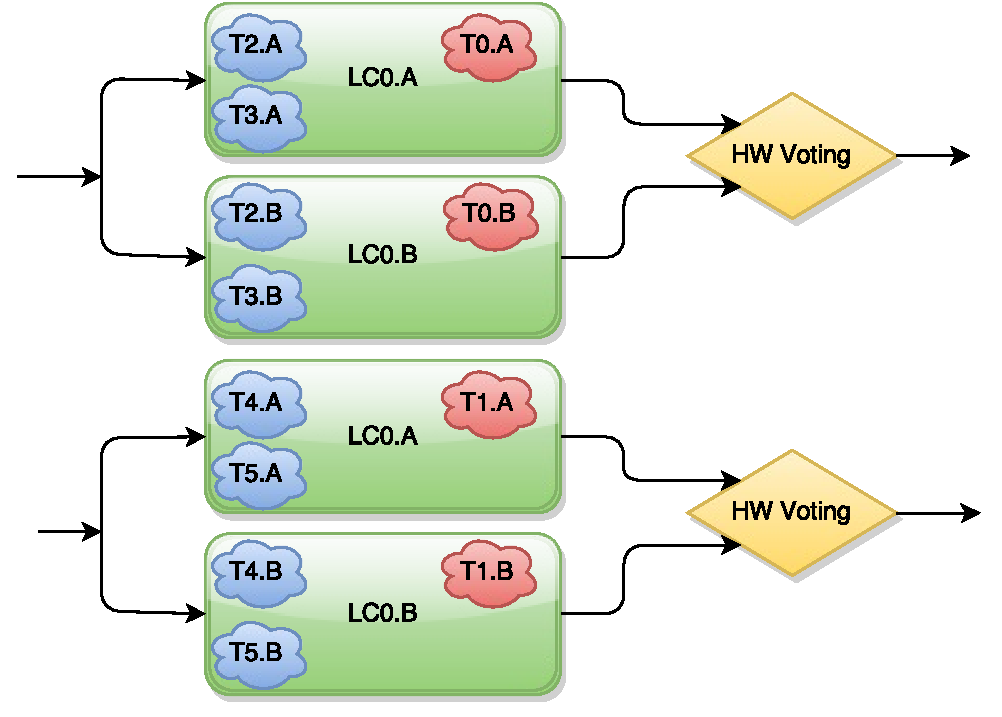
\includegraphics[width=0.42\textwidth]{lockstep.pdf}
}%
\hfill
\subcaptionbox[]{On-demand redundancy \label{f:odr}}[0.45\textwidth]
{
    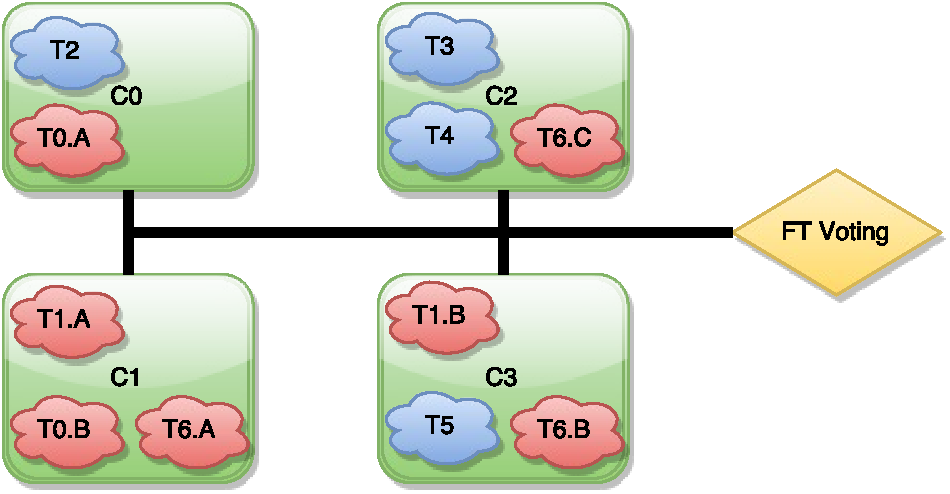
\includegraphics[width=0.42\textwidth]{odr.pdf}
}%
\caption{Different architectures for multicore fault-tolerant systems.}
\label{f:ft-arch}
\end{figure}

	
We make the following {\bf contributions} in this paper:
\td{our contributions}


\section{Related Work}

Research on mixed-criticality systems has flourished in recent years; interested readers are referred to a recent survey~\cite{burns2013mixed}.
Earlier MCS scheduling work, such as AMC~\cite{baruah2011response}, addresses overruns by dropping all LO tasks in HI mode. This assumption is relaxed in \cite{burns2013towards} by allowing LO tasks to continue execution with relaxed parameters (for example, larger period). Later work such as \cite{importance14} propose selecting a subset of LO tasks to continue execution with gradual degradation of service.


Other recent work has begun exploring the scheduling problem in the context of fault-tolerant MCS. For instance, in ~\cite{lin2014scheduling} re-execution slots are reserved for all tasks (both LO and HI). Since faults are rare events, such over-provisioning wastes CPU time and increases hardware costs. We start the system in a mode with no over-provisioning, and only consider re-execution for HI-criticality tasks and in response to faults. In \cite{thekkilakattil2014mixed}, zonal and fault hazard analysis are used to constrain task allocation and re-execution and make offline guarantees for HI tasks. LO tasks are executed if the scenario allows it, but unlike our work, no guarantees are made. In \cite{kang2014static}, a reliability-aware mapping technique is proposed with worst case guarantees for MCS executing on a multiprocessor system-on-chip. However, WCET variation is assumed to be a result of the fault mitigation techniques such as re-execution. In \cite{huang2014scheduling}, the reliability requirements of tasks are accounted for by deriving new values for the HI-criticality tasks' WCETs in the HI mode. None of the three works~\cite{thekkilakattil2014mixed, kang2014static, huang2014scheduling} model the basic MCS premise that HI tasks can have different WCETs coming from, for example, the designer and the certification authority.
The work in~\cite{pathan14} addresses this issue and is similar to our work in considering both fault tolerance and certification requirements for mixed-criticality systems. However, it uses the standard two-mode model of MCS, and LO-criticality tasks are immediately dropped once either a fault or an overrun occurs, compromising QoS for LO tasks.



\section{Assumptions and Notation}
\label{sec:notation}
Our objective is to perform task allocation and scheduling for a set of sporadic mixed-criticality tasks $\Gamma = \{\tau_1,\tau_2,...\}$. The supporting architecture can be single- or multi-core. Tasks are scheduled with fixed priority, and, if the architecture is multicore, with partitioned scheduling. We assume that each core is capable of detecting faults, and that core $\pi$ is characterized by a failure rate $\lambda_{\pi}$ (failures per unit time). Examples of such detection mechanism are acoustic sensors~\cite{UpasaniISCA2014} or lockstep execution~\cite{baleani2003}. 

%In consistency with previous works on fault tolerance in MCS (such as \cite{pathan14}, \cite{kang2014static}, \cite{huang2014scheduling}),

We assume that (a) tasks are independent (i.e., there is no blocking due to shared resources), (b) tasks do not suspend themselves, other than at the end of their computation, (c) the overheads due to context switching, migration, etc., are negligible. Each task $\tau_i$ has a 6-tuple of parameters $\langle L_i, C_i(LO), C_i(HI), T_i, D_i, \gamma_i \rangle$, where:
\begin{itemize}
  \item $L_i \in $  \{LO, HI\} denotes the criticality level of $\tau_i$.
  \item $C_i(LO)$ is the designer-specified WCET for $\tau_i$.
  \item $C_i(HI)$ is the WCET specified by certification authorities.
  \item If $L_i=LO$, $C_i(HI)=C_i(LO)$, otherwise $C_i(LO)\leq C_i(HI)$.
  \item $T_i$ denotes the period (minimum inter-arrival time) of $\tau_i$; tasks have implicit deadlines, i.e., $D_i=T_i$.
\item $\gamma_i$ denotes the priority of $\tau_i$.
  %\item $I_i$ $\epsilon$ (0,1] denotes the importance of task $\tau_i$. HI-criticality tasks have $I_i=1$
\end{itemize}
$u_i$ is the utilization of $\tau_i$, where $u_i(L_i)=C_i(L_i)/T_i$.

Each criticality level is characterized by a maximum probability of failure to which each task of that level must conform, given as a probability of failure per hour (PFH). Sequential re-execution is used as the hardening mechanism to achieve the required reliability level. Each HI task $\tau_i$ must be guaranteed to be schedulable even when it re-executes in response to faults to achieve a failure rate of at most $PFH_i = PFH({HI})$. For LO-criticality tasks, we assume that they do not have specific PFH requirements, hence they do not need to be re-executed when faults occur. This work focuses on the more common transient faults affecting application tasks. Permanent hardware failures and operating system errors are out of the scope of this work.

\subsection{System Operation}
Our system operates as follows:
\begin{enumerate}[topsep=-5pt]
\item  The system starts in the LO mode, where all tasks $i$ execute once ($n_i(LO)=1$) and can run up to $C_i(LO)$.
\item  In LO mode, if any task $i$ executes beyond $C_i(LO)$, the system moves into overrun (OV) mode where all HI-criticality tasks $j$ can safely execute once ($n_j(OV)=1$) up to $C_j(OV) = C_j(HI)$.
\item  Alternatively, in LO mode, if any HI-criticality task experiences a transient fault, the system moves into transient fault (TF) mode where each HI-criticality task $i$ is guaranteed a sufficient number of re-executions to satisfy their reliability requirements as per Eq.~\eqref{eqn:numRexec} ($n_i(TF)>1$). {\it During the mode transition, the required re-executions for HI tasks must be guaranteed to finish before the deadline}. In this way, reliability requirements are met even when the task starts its execution in a mode that does not consider re-executions. The original task and all re-executions are allowed to execute up to $C_i(TF) = C_i(LO)$.
\item  If any of the (re-)executions of a HI-criticality $i$ task in TF mode overruns $C_i(LO)$, the system moves into HI mode. A move to this mode is also possible if the system is in OV mode and a transient fault occurs. In HI mode, HI-criticality tasks $i$ can execute up to $C_i(HI)$ and re-execute $n_i(HI) \ge n_i(TF)$ times.
\end{enumerate}

Modes OV and TF cover the basic cases of task overruns or transient faults by dropping some LO-criticality tasks to allow more time for HI tasks. Both events leading to HI have a low probability, however for highly critical systems, it is important to consider all cases. It is worth noting that in this mode, more re-executions for a HI-criticality task $i$ might be needed than in TF mode ($n_i(HI) \ge n_i(TF)$), because HI-criticality tasks are assumed to run longer ($C_i(HI) \ge C_i(TF)$) and hence may experience more errors.

\subsection{Providing QoS to LO-criticality tasks}

As discussed in Section~\ref{sec:introduction}, one of the criticisms the two-mode MCS model~\cite{baruah2011response, pathan14} is the assumption that all LO tasks are dropped in higher modes~\cite{burns2013mixed}. Our proposed model does not drop all LO tasks in the modes OV, TF, and HI. Instead, LO-criticality tasks are selectively allowed to run in the new mode as long as this does not affect the schedulability of HI tasks. New schedulability analysis that extends AMC to the new model is presented in Section~\ref{sec:schedA}. This analysis provides offline guarantees to all HI tasks and the selected subset of LO tasks. In this way, the designer can be sure of the schedulability of the task set regardless of the runtime scenario. We maximize the number of LO tasks scheduled in each mode; alternatively, the designer may select the LO tasks that continue. 


\subsection{An Illustrative Example}

To illustrate the benefit of the proposed model, we apply the proposed and standard two-mode models to the example task set in Table~\ref{t:example}. The tasks are arranged in priority order (the lowest indexed task has highest priority). We assume the number of executions for HI task $\tau_1$ is $n_1(TF)=n_1(HI)=3$. If an overrun occurs in task $\tau_1$ (Figure \ref{fig:example}a), the system moves into OV mode where $12-4=8$ time units are available to run the LO-criticality tasks in the system. Therefore, we only need to drop one task ($\tau_4$, for example). If $\tau_1$ needs to re-execute due to faults (Figure \ref{fig:example}b), since $n_1(TF)=3$, the system can still schedule one LO task ($\tau_4$). If both faults and overruns occur (Figure~\ref{fig:example}c), the system switches to HI mode, and $\tau_1$ can still run safely with all re-executions. For a two-mode model, any overrun or fault will lead to a scenario similar to Figure~\ref{fig:example}c, and all LO tasks will be dropped immediately.  The four-mode model clearly improves LO task QoS over the two-mode model.

\begin{table}[t!]
\caption{Example Task Set}
\centering

	\begin{tabular}{@{}lcccc@{}}
	\toprule
	& $C(LO)$ & $C(HI)$ & T=D & L 	 \\
	\bottomrule
	$\tau_1$ & 3 & 4 & 12 & HI  \\
	$\tau_2$ & 4 & - & 12 & LO  \\
	$\tau_3$ & 4 & - & 12 & LO  \\
	$\tau_4$ & 1 & - & 12 & LO  \\
	\end{tabular}

\label{t:example}
\end{table}

\begin{figure}[t!]
  \centering
  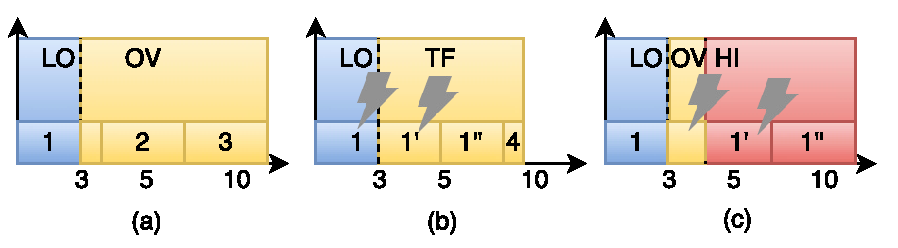
\includegraphics[width=1.0\textwidth]{images/sched_example.pdf}\\
  \caption{An execution trace for the task set in Table \ref{t:example} when (a) an overrun occurs (b) a fault occurs (c) both occur.}
  \label{fig:example}
\end{figure}



\section{Schedulability Analysis}
\label{sec:schedA}

\subsection{Basic Analysis}
\label{sec:basic}
We now present schedulability analysis for the four-mode system by extending the AMC-rtb approach~\cite{baruah2011response} to the proposed new model. The AMC-max schedulability test \cite{baruah2011response} can be similarly extended and is left out due to space limitations.

For a system to be schedulable:
\begin{enumerate}[topsep=-5pt]
\item HI-criticality tasks must be scheduled in all four modes;
\item LO-criticality tasks must be scheduled in the LO mode.
\end{enumerate}
Therefore, for modes OV, TF, and HI we only need to check the schedulability of HI tasks. It is not necessary for the schedulability of the system to guarantee the schedulability of any LO task in these modes. However, through design space exploration, we try to schedule LO tasks in these modes as long as the overall system schedulability is not affected.

For LO mode the response time of a task $\tau_i$ is given by:
\begin{equation}
R_i^{(LO)}= C_i(LO)+\sum_{j \in hp(i)}\Big\lceil\frac{R_i^{(LO)}}{T_j}\Big\rceil \cdot C_j(LO)
\label{eq:mode1}
\end{equation}
%
where $hp(i)$ is the set of tasks on $\tau_i$'s processor that have higher priority than $\tau_i$ (including both HI and LO tasks).

When evaluating schedulability in mode TF, we need to consider two cases.  First, we need to consider the stable case: the given HI-criticality task itself and higher priority tasks. Second, we also need to verify that the mode change LO-to-TF does not cause the given task to miss its deadline. The response time of a task in the mode change is larger than in the stable mode, since in addition to the task itself and higher priority tasks executing in mode TF, we need to consider the effect of LO-criticality tasks that may be dropped in TF but have not finished executing. The worst case response time of a task in TF is hence the response time of the mode change and is given by Equation~\eqref{eq:mode2}.
%
\begin{equation}\label{eq:mode2}
\begin{aligned}
R_i^{(TF)} & = n_i(TF) \cdot C_i(LO) \\
&  +\sum_{j \in hpC(TF,i)}\Big\lceil\frac{R_i^{(TF)}}{T_j}\Big\rceil \cdot n_j(TF) \cdot C_j(LO) \\
&  +\sum_{k \in hp(i)-hpC(TF,i)}\Big\lceil\frac{R_i^{(LO)}}{T_k}\Big\rceil \cdot C_k(LO)
\end{aligned}
\end{equation}

In TF, we need to take into account task re-executions for HI-criticality tasks $j$, hence $C_j(LO)$ values are multiplied by the number of re-executions $n_j(TF)$. $hpC(TF,i)$ is the set of higher priority continuing tasks (i.e., tasks that continue to execute in the current mode TF). This set of tasks contains all HI tasks and those LO tasks selected to continue.  The last summation considers the tasks that get dropped in the LO-to-TF mode change (in the set $hp(i)-hpC(TF,i)$). These tasks can only execute up to $R_i^{(LO)}$ since a mode change must occur before $R_i^{(LO)}$, otherwise $\tau_i$ would have terminated before the mode change.  Since only LO tasks are allowed to be dropped, we use $C_k(LO)$ and $n_k=1$ here.

%Note that $hp(i)=hpC(LO,i)$ $\cup$ $hpD(LO,i)$
%The set $hpD(LO,i)$ is the set of high priority dropped tasks (i.e. tasks that execute in mode LO but get dropped in the current mode). This set contains only LO tasks as HI tasks are never dropped.

The response time for mode OV can be similarly calculated. However, HI tasks can execute up to $C(HI)$ and no re-executions are considered ($n=1$ for all tasks). The response time in mode OV is given by:
%
\begin{equation}\label{eq:mode3}
\begin{aligned}
R_i^{(OV)} &  = C_i(L_i)+\sum_{j \in hpC(OV,i)}\Big\lceil\frac{R_i^{(OV)}}{T_j}\Big\rceil \cdot C_j(L_j) \\
&  +\sum_{k \in hp(i)-hpC(OV,i)}\Big\lceil\frac{R_i^{(LO)}}{T_k}\Big\rceil \cdot C_k(LO)
\end{aligned}
\end{equation}
% \vspace{-4mm}
% where $coj(i,y,z)$ is the set of carry-over jobs in the mode change from mode y to mode z on $\tau_i$'s processor. i.e. the set of tasks that are allocated to $\tau_i$'s processor in mode y but allocated to another processor or dropped in mode y.

In mode HI, we need to consider both overruns ($C_i(HI)$) and re-execution ($n_i(HI) \ge 1$). Transitions to the HI mode can originate from either TF or OV mode. Both mode changes need to be verified. The worst case scenario occurs when we encounter two consecutive mode changes in quick succession (LO-to-TF-to-HI or LO-to-OV-to-HI).

Focusing on the LO-to-TF-to-HI mode change first (Equation~\eqref{eq:mode4a}), the task $\tau_i$ under analysis and the high priority continuing tasks in mode HI $hpC(HI, i)$ are allowed to execute $n$ times (first and second terms on the right hand side of the equation). For tasks that are allowed to continue in TF mode but dropped in HI mode (i.e., in the set $hpC(TF,i)-hpC(HI,i)$), we assume that the mode change from TF to HI has to happen before $R_i^{(TF)}$ (third term). Finally, for the remaining tasks in $hp(i)$ (i.e. tasks that started in LO and got dropped in TF), the interference is bounded by the fact that the mode change from LO to TF has to happen before $R_i^{(LO)}$ (last term). Note that we do not consider re-executions for those dropped tasks $(n_k=n_l=1)$ as they are all LO-critical.
%
%{\bf In modes 3 and 4, we need to make sure that the task and all its replicas finish by the deadline. To make sure of that, they are treated as a single unit within the schedulability analysis. This can done by performing the analysis of a task $\tau_i$ with $n_i.C_i$ instead of $C_i$. For LO-criticality tasks the two values are equal.}
\begin{equation}\label{eq:mode4a}
\begin{aligned}
R_i^{(HIa)} & = n_i(HI) \cdot C_i(L_i) \\
&  +\sum_{j \in hpC(HI,i)}\Big\lceil\frac{R_i^{(HIa)}}{T_j}\Big\rceil \cdot n_j(HI) \cdot C_j(L_j) \\
&  +\sum_{k \in hpC(TF,i)-hpC(HI,i)}\Big\lceil\frac{R_i^{(TF)}}{T_k}\Big\rceil \cdot C_k(LO)\\
&  +\sum_{l \in hp(i)-hpC(TF,i)}\Big\lceil\frac{R_i^{(LO)}}{T_l}\Big\rceil \cdot C_l(LO)
\end{aligned}
\end{equation}

Similarly, the task response time of $\tau_i$ for LO-to-OV-to-HI transition is presented in Equation~\eqref{eq:mode4b}:
\begin{equation}\label{eq:mode4b}
\begin{aligned}
R_i^{(HIb)} & = n_i(HI) \cdot C_i(L_i) \\
&  +\sum_{j \in hpC(HI,i)}\Big\lceil\frac{R_i^{(HIb)}}{T_j}\Big\rceil \cdot n_j(HI) \cdot C_j(L_j) \\
&  +\sum_{k \in hpC(OV,i)-hpC(HI,i)}\Big\lceil\frac{R_i^{(OV)}}{T_k}\Big\rceil \cdot C_k(LO)\\
&  +\sum_{l \in hp(i)-hpC(OV,i)}\Big\lceil\frac{R_i^{(LO)}}{T_l}\Big\rceil \cdot C_l(LO)
\end{aligned}
\end{equation}
The response time of $\tau_i$ in HI mode is the maximum of the two possible transitions:
\begin{equation}
R_i^{(HI)}= \max(R_i^{(HIa)},R_i^{(HIb)})
\label{eq:mode4}
\end{equation}



\section{Extending Response Time Analysis to ODR}
\label{s:multicorerta}
	We will extend the analysis on lockstep (LS) to support three types of ODR. The four scenarios (including lockstep) are shown in Figure~\ref{f:ftm}. 
	In (a), LS execution occurs when a node has internal mechanisms for detecting but not correcting errors. 
	An error simply results in a re-execution on that node, as previously discussed. 	
	In (b), dual modular redundancy (DMR) replicates a thread on two cores that cannot detect errors by themselves. 
	The task must be re-executed if the executions do not match according to some external comparison or voting mechanism.
	In (c), triple modular redundancy (TMR) replicates a thread on three cores that cannot detect errors. 
	If an error occurs, the majority answer is taken from the three replicas and no re-execution is required (the system assumes only one replica may fail at a time).
	Finally, in (d), passive replication is similar to TMR but the final replica does not execute if the first two copies return the same result. 


\addfigure{0.55}{ftm.pdf}{The 4 fault tolerance mechanisms supported by the proposed MCFTS analysis}{f:ftm}
	
	Each technique is expressed in the new analysis by three parameters: a task set transformation, mapping constraints, and a re-execution profile denoted by $N$.
	The task set transformation represents each replica explicitly in the task set. 
	Consider the example task set in Table~\ref{t:transform}. 
	Lockstep does not introduce any replicas to the system and does not require any transformation of the task set. 
	DMR requires one replica to be added to the task set while TMR and PR require two replicas to be added.
	
	Constraints must be added to the problem for the processors $\pi_i$ assigned to $\tau_i$ in order to properly reflect the semantics of the different techniques. 
	The constraints shown in the table ensure that the replicas are not assigned to the same core. 
	These constraints will be useful in the mapping stage.
	
	
\begin{table*}
\centering
\caption{Task set transformations}
\label{t:transform}
	\begin{subtable}{0.3\textwidth}
		\caption{Example task set}
		\begin{tabular}{@{}l|cccc@{}}
		\toprule
		& C(LO) & C(HI) & T=D & L 	 \\\bottomrule
		$\tau_1$ & 5 & 10 & 25 & HI  \\
		$\tau_2$ & 5 & - & 20 & LO  \\
		\multicolumn{5}{c}{ } \\
		\multicolumn{5}{c}{ } \\
		\end{tabular}
	\end{subtable} 
	\begin{subtable}{0.3\textwidth}
		\caption{DMR transformation}
		\begin{tabular}{@{}l|cccc@{}}
		\toprule
				& C(LO) & C(HI) & T=D & L	 \\\bottomrule
		$\tau_1$ & 5 & 10 & 25 & HI  \\
		$\tau_{1.1}$ & 5 & 10 & 25 & HI  \\
		$\tau_2$ & 5 & - & 20 & LO  \\
		\multicolumn{5}{c}{$\pi_1 \ne \pi_{1.1}$}
		\end{tabular}
	\end{subtable}
	\begin{subtable}{0.3\textwidth}
		\caption{TMR transformation}
		\begin{tabular}{@{}l|cccc@{}}
		\toprule
				& C(LO) & C(HI) & T=D & L	 \\\bottomrule
		$\tau_1$ & 5 & 10 & 25 & HI  \\
		$\tau_{1.1}$ & 5 & 10 & 25 & HI  \\
		$\tau_{1.2}$ & 5 & 10 & 25 & HI  \\
		$\tau_2$ & 5 & - & 20 & LO  \\
		\multicolumn{5}{c}{$\pi_1 \ne \pi_{1.1} \ne \pi_{1.2}$}
		\end{tabular}
	\end{subtable} 
	\begin{subtable}{0.3\textwidth}
		\caption{PR replication}
		\begin{tabular}{@{}l|cccc@{}}
		\toprule
		& C(LO) & C(HI) & T=D & L	 \\\bottomrule
		$\tau_1$ & 5 & 10 & 25 & HI  \\
		$\tau_{1.1}$ & 5 & 10 & 25 & HI  \\
		$\tau_{1.2}$ & 5 & 10 & 25 & HI  \\
		$\tau_2$ & 5 & - & 20 & LO  \\
		\multicolumn{5}{c}{$\pi_1 \ne \pi_{1.1}$}
		\end{tabular}
	\end{subtable}
\end{table*}


	The re-execution variable $n_i$ has been generalized into the vector:
\begin{equation}
	N_i=<n_i(LO),n_i(OV),n_i(TF),n_i(HI)>
\end{equation} 
	The $N$ for each mode is shown in Table~\ref{t:reex} and the updated equation for the OV mode response time are given by the following equations:
	\begin{equation}
\begin{aligned}
R_i^{(OV)} =
\begin{dcases*}
C_i(L_i)\color{red} \color{black}+\sum_{j \in hpC(OV,i)}\Big\lceil\frac{R_i^{(OV)}}{T_j}\Big\rceil \cdot C_j(L_j) \\
\hspace{0.3cm} +\sum_{k \in hp(i)-hpC(OV,i)}\Big\lceil\frac{R_i^{(LO)}}{T_k}\Big\rceil \cdot C_k(LO), &  $n_i(OV)>0$ \\
	0, \\ 	& $n_i(OV)=0$
\end{dcases*}
   \end{aligned}
\end{equation}
	We note that all techniques have $n(LO)$ and $n(OV)$ values of either 0 or 1. When $n=0$, the task is not executing and the response time is simply 0. The same is true for LO mode.
	
	For example, TMR has $N=<1,1,1,1>$. This means that in all modes, any task using TMR will have $n=1$ which in effect signals that no re-executions are required. For PR, one replica executes one time in all modes and the other only executes in the case of a fault (hence only executes once in TF or HI modes).

	\begin{table}
\caption{Re-execution profiles for the fault tolerance mechanisms}
\label{t:reex}
\centering
	\begin{tabular}{@{}l|c@{}}
	\toprule
	Technique & Profile ($N$) \\
	\bottomrule
	LS & $<1,2,1,2>$ \\
	DMR & $<1,2,1,2>$ \\
	TMR & $<1,1,1,1>$ \\
	PR & $<1,1,1,1>$ and $<0,1,0,1>$ \\
	\end{tabular}
\end{table} 	

\section{Design Space Exploration}
\label{s:dse}


\subsection{Two Stage GA}
	The mapping and scheduling algorithm follows the procedure used in \cite{bolchini2013reliability} and \cite{kang2014reliability}. 
	Two stages of genetic algorithms (GA), implemented using JGAP \cite{jgap}, are used to explore both the techniques used to harden each task and the core assignment for each task and its replicas. 
	The basic flow is shown in Figure~\ref{f:dse}. 
	The Reliability Aware (RA) stage is responsible for mapping a fault tolerance mechanism to each task. 
	The RA stage then generates a chromosome structure for the Mapping and Scheduling (MS) stage. 
	The MS stage attempts to find an allocation for each task onto a core that maximizes the average QoS across all modes in the system using the response time analysis from Section~\ref{s:mcfts}.
	It is necessary to define the problem in terms of a chromosome for each stage.
	
\addfigure{0.6}{dse.pdf}{Overview of DSE workflow using nested genetic algorithm searches}{f:dse}
	
	The chromosome in the RA stage has one integer gene for each task representing a fault tolerance mechanism. 
	For instance, consider a task set with two HI tasks ${\tau_1,\tau_2}$ being mapped onto a platform that supports LS, DMR and TMR - the chromosome would consist of two genes each limited to integers in the range $[0,2]$. 
	
	The RA fitness function (FF) must determine the fitness (QoS) for each configuration of fault tolerance mechanisms. 
	The FF creates a new task set using the transformations in Table~\ref{t:transform} as well as the necessary constraints. 
	The FF then creates a chromosome template for the MS stage based on the transformed task set. 
	Given the number of processors that a task can be mapped to, $n$, it is possible to determine for each FTM a mapping rule that generates a unique configuration from an integer. 
% 	Each gene in the chromosome is an integer representing a unique allocation for a task and its replicas. 
	It is important that the task and replicas are represented by a single gene or else most chromosomes will result in illegal configurations after mutation and crossover. 
	Table~\ref{t:mschrom} shows the number of configurations for each type of FTM and how to derive a unique allocation as a function of the number of candidate cores ($n$) from a random integer $x < n$. 
	The conversion rule provides an index into an ordered list of the cores. A core is removed from the list once it is allocated.
	
	For example, consider a task and two replicas using TMR in a sytem with 5 processing cores. 
	All three tasks must go on different cores. 
	The number of configurations is $5 \cdot 4 \cdot 3 = 60$. 
	The GA will generate a random integer in the range $[0,59]$ representing a unique mapping of the three tasks onto the system, say 47. 
	The number 47 is converted using the TMR rule to $(47/(4\cdot3),(47\bmod(4\cdot3))/3,47\bmod3) = (3,3,1)$. 
	Suppose the core list is $\{\pi_1,\pi_2,\pi_3,\pi_4,\pi_5\}$. 
	The first copy is allocated to $\pi_3$ and $\pi_3$ is then removed from the list. 
	The next copy is assigned to $\pi_4$ (now at index 3) and the third copy is assigned to $\pi_1$. 
	
	\begin{table*}
\caption{Rules for generating unique MS configurations from an integer $x$ for $n$ cores}
\label{t:mschrom}
\centering
	\begin{tabular}{@{}l|cc@{}}
	\toprule
	Technique & Configurations & Conversion Rule \\
	\bottomrule
	none & $n$ & $(x)$\\
	LS & $n$ & $(x)$ \\
	DMR & $n(n-1)$ & $(\frac{x}{n-1},x\bmod{(n-1)})$ \\
	TMR & $n(n - 1)(n-2)$ & $(\frac{x}{(n - 1)(n - 2)}, \frac{x\bmod ((n-1)(n-2))}{n-2}, x \bmod (n-2))$ \\
	PR & $n^2 (n-1)$ & $(\frac{x}{n(n - 1)}, \frac{x \bmod (n(n-1))}{n-1}, x \bmod (n-1))$ \\
	\end{tabular}
\end{table*} 	

	A unique MS stage is instantiated for each chromosome in the RA stage population. 
	The MS stage generates a population based on the chromosome built by the RAFF. 
	The MSFF builds each chromosome into a schedule and passes it along to the schedulability analysis. 
	If the system is schedulable then the chromosome is assigned a fitness value equal to the average QoS across all four modes (defined as percentage of LO tasks that have not been dropped).
	If the analysis fails then the chromosome is assigned a fitness value of 0.
	
	\section{Experimental Results}
	
	\td{Three figures are interesting because\ldots}
% 	\addfigure{0}{name}{caption}{label}
	\addfigure{0}{mc-plat-qos-hi.jpg}{ODR provides better QoS in multicore systems}{f:mc-mec-qos-hi}
	\addfigure{0}{mc-mec-qos-hi}{Combining several ODR techniques improves QoS}{f:mc-mec-qos-hi}
	\addfigure{0}{mc-mec-sched}{Combining several ODR techniques improves schedulability}{f:mc-mec-sched}
	
\section{Conclusion}
\label{sec:conclusion}


\section*{Acknowledgments}

% %\bibliographystyle{IEEEtran}
% %\bibliography{ftmc}

\begin{thebibliography}{10}
\providecommand{\url}[1]{#1}
\csname url@samestyle\endcsname
\providecommand{\newblock}{\relax}
\providecommand{\bibinfo}[2]{#2}
\providecommand{\BIBentrySTDinterwordspacing}{\spaceskip=0pt\relax}
\providecommand{\BIBentryALTinterwordstretchfactor}{4}
\providecommand{\BIBentryALTinterwordspacing}{\spaceskip=\fontdimen2\font plus
\BIBentryALTinterwordstretchfactor\fontdimen3\font minus
  \fontdimen4\font\relax}
\providecommand{\BIBforeignlanguage}[2]{{%
\expandafter\ifx\csname l@#1\endcsname\relax
\typeout{** WARNING: IEEEtran.bst: No hyphenation pattern has been}%
\typeout{** loaded for the language `#1'. Using the pattern for}%
\typeout{** the default language instead.}%
\else
\language=\csname l@#1\endcsname
\fi
#2}}
\providecommand{\BIBdecl}{\relax}
\BIBdecl


\bibitem{burns2013mixed}
A.~Burns and R.~Davis, ``Mixed criticality systems-a review,'' \emph{Department
  of Computer Science, University of York, Tech. Rep}, 2015.

\vspace{-0.5mm}
\bibitem{baruah2011response}
S.~Baruah, A.~Burns, and R.~Davis, ``Response-time analysis for mixed
  criticality systems,'' in \emph{32nd IEEE Real-Time Systems Symposium}, 2011.


\vspace{-0.5mm}
\bibitem{baleani2003}
M.~Baleani, A.~Ferrari, L.~Mangeruca, A.~Sangiovanni-Vincentelli, M.~Peri, and S.~Pezzini,
 ``Fault-tolerant platforms for automotive safety-critical applications,'' in \emph{International conference
 on Compilers, architecture and synthesis for embedded systems}, 2003.



\vspace{-0.5mm}
\bibitem{kang2014static}
S.~Kang, H.~Yang, S.~Kim, I.~Bacivarov, S.~Ha, and L.~Thiele,
``Static Mapping of Mixed-Critical Applications for Fault-Tolerant MPSoCs,''
in \emph{Design Automation Conference}, 2014.


\vspace{-0.5mm}
\bibitem{huang2014scheduling}
P.~Huang, H.~Yang, and L.~Thiele, ``On the scheduling of fault-tolerant
  mixed-criticality systems,'' in \emph{Design Automation Conference}, 2014.

\vspace{-0.5mm}
\bibitem{pathan14}
R.~Pathan, ``Fault-tolerant and real-time scheduling for mixed-criticality systems,''
  \emph{Real-Time Systems}, 50(4):509--547, 2014.

\vspace{-0.5mm}
\bibitem{yip2014relaxing}
E.~Yip, M.~M. Kuo, P.~S. Roop, and D.~Broman,
``Relaxing the synchronous
  approach for mixed-criticality systems,'' in \emph{IEEE Real-Time and Embedded
  Technology and Applications Symp.}, 2014.

\vspace{-0.5mm}
 \bibitem{burns2013towards}
A.~Burns and S.~Baruah, ``Towards a more practical model for mixed criticality
  systems,'' \emph{Workshop on Mixed Criticality Systems}, 2013.

\vspace{-0.5mm}
 \bibitem{importance14}
T.~Fleming and A.~Burns, ``Incorporating the notion of importance into mixed
  criticality systems,'' \emph{Workshop on Mixed Criticality  Sys.}, 2014.


\vspace{-0.5mm}
\bibitem{lin2014scheduling}
J.~Lin, A.~M. Cheng, D.~Steel, and M.~Y.-C. Wu, ``Scheduling mixed-criticality
  realtime tasks with fault tolerance,'' in \emph{Workshop on Mixed
  Criticality Systems}, 2014.


\vspace{-0.5mm}
\bibitem{thekkilakattil2014mixed}
A.~Thekkilakattil, R.~Dobrin, and S.~Punnekkat, ``Mixed criticality scheduling
  in fault-tolerant distributed real-time systems,'' in \emph{International Conference on Embedded Systems}, 2014.


\vspace{-0.5mm}
\bibitem{UpasaniISCA2014}
G.~Upasani, X. Vera, and A. Gonz\'{a}lez,
``Avoiding core's DUE \& SDC via acoustic wave detectors and tailored error containment and recovery,''
in \emph{Int. Symposium on Computer Architecuture}, 2014.


\vspace{-0.5mm}
\bibitem{lafrieda2007utilizing}
C.~LaFrieda, E.~Ipek, J.~F. Martinez, and R.~Manohar, ``Utilizing dynamically
 coupled cores to form a resilient chip multiprocessor,'' in \emph{IEEE/IFIP Int.
 Conf. on Dependable Systems and Networks}, 2007.



\vspace{-0.5mm}
\bibitem{meyer2011}
B.~H.~Meyer, B.~H.~Calhoun,  J.~Lach, and K.~Skadron,
``Cost-effective safety and fault localization using distributed temporal redundancy,''
\emph{Compilers, architecture and synthesis for embedded systems}, 2011.


\vspace{-0.5mm}
\bibitem{ElesDATE2008}
P. Eles, V. Izosimov, P. Pop, and P.~Zebo, ``Synthesis of Fault-Tolerant Embedded Systems,''
\emph{Design, Automation and Test in Europe}, 2008.


\vspace{-0.5mm}
\bibitem{bini2005measuring}
E.~Bini and G.~C. Buttazzo, ``Measuring the performance of schedulability
  tests,'' \emph{Real-Time Systems}, 30(1-2):129--154, 2005.

\vspace{-0.5mm}
\bibitem{zaidaspdac15}
Z.~Al-bayati, Q.~Zhao, A.~Youssef, H.~Zeng, and Z.~Gu, ``Enhanced partitioned scheduling of Mixed-Criticality Systems on multicore platforms,'' \emph{Asia and South Pacific Design Automation Conf.}, 630--635, 2015.






\end{thebibliography}




% that's all folks
\end{document}


